% -- Document configuration
\documentclass{article}

% -- Input and language settings
% \usepackage[utf8]{inputenc}
\usepackage[spanish]{babel}
\decimalpoint                             % From babel package to use points instead of commas in decimals

% -- Page and line settings
\usepackage{geometry}
\geometry{letterpaper, 
    % margin=2cm, 
    left=3cm, right=3cm,
    top=1.2cm, bottom=1.2cm,
    includefoot, 
    includehead}
\renewcommand{\baselinestretch}{1.2}

% -- Required packages
\usepackage{xcolor}
\usepackage[many]{tcolorbox}
\usepackage{mathtools,amsfonts,amsmath}     % Loads amsmath if not already loaded
\allowdisplaybreaks                         % To allow page breaks if equations are too long
\usepackage[parfill]{parskip}               % No indent and separation lines for paragraphs
\usepackage{cancel}                         % To cancel math terms
\usepackage[shortlabels]{enumitem}          % To handle enumerations
\usepackage{tikz}
\usetikzlibrary{automata, arrows.meta, positioning}
\usepackage[mode=buildnew]{standalone}      % To import figures in standalone files
\usepackage[hidelinks]{hyperref}
\usepackage[spanish]{cleveref}              % To use autocompleted reference labels, language must be change as in babel package
\usepackage{caption}                        % Caption and subcaption to allow subfigures
\usepackage{subcaption}
\usepackage{float}                          % To specify the location of figures
\usepackage{multicol}                       % To use multicolumns
\usepackage[bottom]{footmisc}               % To locate footnotes at the bottom

% -- Title and heading settings
\usepackage{titling}
\usepackage{fancyhdr}
\pagestyle{fancy}

% -- Code and code formatting
\usepackage{minted}                         % To insert code
\usemintedstyle[julia]{gruvbox-light}       % Code theme and language
\definecolor{bg}{rgb}{0.98, 0.97, 0.88}     % Code block background

\usepackage{fontspec}                       % To allow the use of monospace fonts
\setmonofont{JuliaMono}[Path=./codefonts/, Extension=.ttf, UprightFont=*-Regular, ItalicFont=*-RegularItalic, Scale=0.75]

\usepackage{fancyvrb}                       % To change line number font
\renewcommand{\theFancyVerbLine}{\textcolor{gray}{\footnotesize\texttt{\arabic{FancyVerbLine}}}}

\definecolor{light-gray}{gray}{0.95}        % Color, box and style to show small code thingys inside normal text
\newcommand{\code}[1]{\colorbox{light-gray}{\texttt{#1}}}

% -- Bilbiography preferences
\usepackage[square,numbers]{natbib}
\bibliographystyle{unsrt}

% -- Footnotes without numbering
\newcommand\nnfootnote[1]{%
  \begin{NoHyper}
  \renewcommand\thefootnote{}\footnote{#1}%
  \addtocounter{footnote}{-1}%
  \end{NoHyper}
}

% -- Theorems
\newtheorem{theorem}{Theorem}

\lhead{\theinstitution\ -- \thedepartment}
\chead{}
\rhead{Programación para la IA\ -- \thetitle}
\lfoot{}
\cfoot{\thepage}
\rfoot{}

% -- Problem solution
\newenvironment{solution}
{\begin{quote}
\textbf{Solución:}\medskip

}
{

\hfill\rule{0.5\textwidth}{0.5pt}
\end{quote}}

% -- Equation result
\newcommand{\result}[1]
{
\tcbhighmath[colframe=white, colback=gray!15, sharp corners]
{#1}
}

% -- Function definitions
\newcommand{\dprod}[2]{{#1} \cdot {#2}}
\newcommand{\txtgray}[1]{\textcolor{gray}{#1}}

% -- Author information
\title{Actividad 5}
\author{Leonardo Flores Torres}
\newcommand\theinstitution{Universidad Veracruzana}
\newcommand\thedepartment{Inteligencia Artificial}
\newcommand\thecourse{Programación para la Inteligencia Artificial}

% -- Paths
% \newcommand\codelists{../programs/lists.rkt}

% Remove red color boxes of "syntax errors" in minted
\AtBeginEnvironment{minted}{%
  \renewcommand{\fcolorbox}[4][]{#4}}

% -- Document
\begin{document}

\thispagestyle{empty}

% Title
\begin{center}
\textsc{\theinstitution}\\[2mm]

\thedepartment

\rule{0.6\textwidth}{0.5pt}\\[2mm]

\thecourse \\[4mm]

{\Large \textbf{\thetitle}}\\[2mm]

\theauthor \\[2mm]

{\small \today}
\end{center}
\medskip

% --

Build a DFA $M_C$ that recognizes the regular language $C = \left\{w\ |\ w\ \text{has at least 3 $a$'s and at least 2 $b$'s} \right\}$ and has an alphabet $\Sigma = \left\{a, b\right\}$.

\begin{solution}
    To move forward with the solution of the problem, it is important to mention the following theorem:
    \begin{theorem}
        The class of regular languages is closed under the intersection operation.
    \end{theorem}

    \begin{figure}[ht!]
        \centering
        \begin{subfigure}[b]{0.4\textwidth}
            \centering
            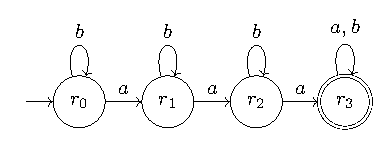
\includegraphics{automaton_a}
            \caption{Automaton $M_A$ that recognizes $A$.}
            \label{fig:automaton_a}
        \end{subfigure}
        \begin{subfigure}[b]{0.4\textwidth}
            \centering
            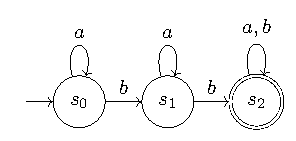
\includegraphics{automaton_b}
            \caption{Automaton $M_B$ that recognizes $B$.}
            \label{fig:automaton_b}
        \end{subfigure}
        \caption{Automata in which the automaton $M_C$ is divided into.}
    \end{figure}

    Lets us assume that the language $C$ of the automaton $M_C$ is a regular language. In fact, \textit{a language is called a regular language if some finite automaton recognizes it}\footnote{Introduction to the Theory of Computation - Michael Sipser.}. The finite automaton $M_C$ and the langauge it recognizes, $C$, can be regarded as the intersection of two regular languages $A$ and $B$ corresponding to the automata $M_A$ and $M_B$, respectively. The regular language $C$ was divided to take advantage of the intersection theorem between regular languages and to ease its construction. The regular languages $A$ and $B$ can be expressed as,
    \begin{equation*}
        \begin{array}{l l}
            A & = \left\{w\ |\ w\ \text{has at least 3 $a$'s}\right\}, \\
            B & = \left\{w\ |\ w\ \text{has at least 2 $b$'s}\right\}.
        \end{array}
    \end{equation*}
    The diagram of the automaton $M_A$ is shown in \cref{fig:automaton_a}, and it is described by the 5-tuple $(Q_A,\Sigma,\delta_A,r_0,F_A)$ where
    \begin{equation*}
        \begin{array}{l l}
            Q_A & = \left\{r_0, r_1, r_2, r_3\right\}, \\
            F_A & = \left\{r_3\right\}.
        \end{array}
    \end{equation*}
    The alphabet $\Sigma$ is the same for both $M_A$ and $M_B$. Additionally, the transition function has the same form, i.e., $\delta_I : Q_I \times \Sigma \to Q_I$ where $Q_I = Q_A, Q_B$. Similarly, the diagram of $M_B$ is shown in \cref{fig:automaton_b} and it is described by the 5-tuple $(Q_B, \Sigma, \delta_B, s_0, F_B)$ where,
    \begin{equation*}
        \begin{array}{l l}
            Q_B & = \left\{s_0, s_1, s_2\right\}, \\
            F_B & = \left\{s_2\right\}.
        \end{array}
    \end{equation*}
    The transition tables that describe $\delta_A : Q_A \times \Sigma \to Q_A$ and $\delta_B : Q_B \times \Sigma \to Q_B$ are:
    \begin{equation*}
        \begin{array}{c c}
            \begin{array}[t]{c | c c}
                Q_A \backslash \Sigma & a & b \\
                \hline
                r_0 & r_1 & r_0 \\
                r_1 & r_2 & r_1 \\
                r_2 & r_3 & r_2 \\
                r_3 & r_3 & r_3
            \end{array} \quad & \quad 
            \begin{array}[t]{c | c c}
                Q_B \backslash \Sigma & a & b \\
                \hline
                s_0 & s_0 & s_1 \\
                s_1 & s_1 & s_2 \\
                s_2 & s_2 & s_2
            \end{array}
        \end{array}
    \end{equation*}

    In the same way, the 5-tuple that describes $M_C$ is $(Q_C, \Sigma, \delta_C, t_0, F_C)$ has a set of states such that
    \begin{equation*}
        \begin{array}{l l}
            Q_C & = \left\{t_{i,j} = (r_i, s_j)\ |\ r_i \in Q_A \land s_j \in Q_B\right\}, \\
            & = Q_A \times Q_B\ . \\
        \end{array}
    \end{equation*}
    The symbol $t_{i,j}$ was used to denote $t_{i,j} = (r_i, s_j)$ for convenince of use throughout this assignment.

    Also, the alphabet is the same as the one originally defined, and the initial state is now a 2-tuple $t_{0,0} = (r_0, s_0)$. On the other hand, the accept states, for the intersection, are given by
    \begin{equation*}
        \begin{array}{l l}
            F_C & = \left\{t_{i,j} = (r_i, s_j)\ |\ r_i \in F_A \land s_j \in F_B\right\} \\
            & = F_A \times F_B\ , \\
            & = \{r_3\} \times \{s_2\}\ , \\
            & = \{(r_3, s_2)\}\ .
        \end{array}
    \end{equation*}
    In contrast with the accept states coming from the union of two regular languages, the accept states in the intersection are only those whose both elements in the 2-tuple also belong to accept states.

    Now, taking our attention to the transition function, it is defined as
    \begin{equation*}
        \delta_C\left((r_i, s_j),\ a\right) = \left(\delta_A(r_i, a),\ \delta_B(s_j, a)\right)\ ,
    \end{equation*}
    where $(r_i, s_i) \in Q_C$. Thus, it is possible to contruct the transition table based on the individual transitions from $\delta_A$ and $\delta_B$, as shown below:
    % To make the columns come closer and save border space
    \setlength{\columnsep}{-1.5cm}
    \begin{multicols}{2}
        \begin{equation*}
            \begin{array}{c | c c}
                Q_C \backslash \Sigma & a & b \\
                \hline
                (r_0, s_0) & (r_1, s_0) & (r_0, s_1) \\
                (r_0, s_1) & (r_1, s_1) & (r_0, s_2) \\
                (r_0, s_2) & (r_1, s_2) & (r_0, s_2) \\
    
                (r_1, s_0) & (r_2, s_0) & (r_1, s_1) \\
                (r_1, s_1) & (r_2, s_1) & (r_1, s_2) \\
                (r_1, s_2) & (r_2, s_2) & (r_1, s_2) \\
    
                (r_2, s_0) & (r_3, s_0) & (r_2, s_1) \\
                (r_2, s_1) & (r_3, s_1) & (r_2, s_2) \\
                (r_2, s_2) & (r_3, s_2) & (r_2, s_2) \\
    
                (r_3, s_0) & (r_3, s_0) & (r_3, s_1) \\
                (r_3, s_1) & (r_3, s_1) & (r_3, s_2) \\
                (r_3, s_2) & (r_3, s_2) & (r_3, s_2) \\
            \end{array}
        \end{equation*}
        \columnbreak
        \begin{figure}[H]
            \centering
            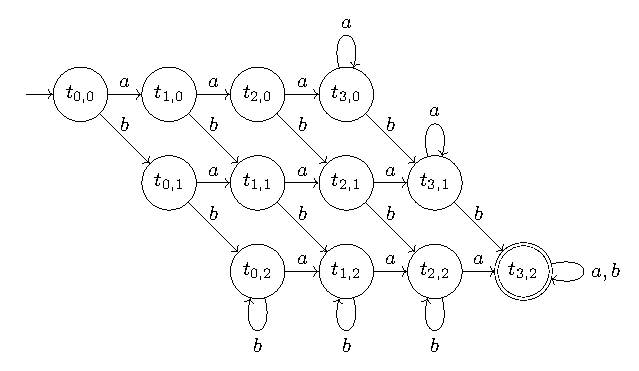
\includegraphics[scale=0.85]{automaton_c}
            \caption{Automaton $M_C$ that recognizes the regular language which is an intersection of the regular languages A and B.}
            \label{fig:automaton_c}
        \end{figure}
    \end{multicols}
    $\therefore$ The resulting DFA $M_C$ is shown in \cref{fig:automaton_c} and it recognizes the regular language $C$ which was constructed as an intersection of the regular languages $A$ and $B$ from $M_A$ and $M_B$, respectively.
\end{solution}
\end{document}